\documentclass[11pt,twoside,UTF8]{ctexart}
\usepackage{graphicx}
\usepackage{geometry}
\geometry{left=1.0cm,right=1.0cm,top=2.5cm,bottom=2.5cm}
\begin{document}
旋转变换,顾名思义就是一个图形绕着一个点转,
而转之前和转之后有部分相同的性质,在我们学习
了等腰三角形后,可以利用相等的边旋转与另一边
重合得到一部分性质,接下来我将用例题解释这一
观点。\\
\begin{figure}[ht]
    \centering
    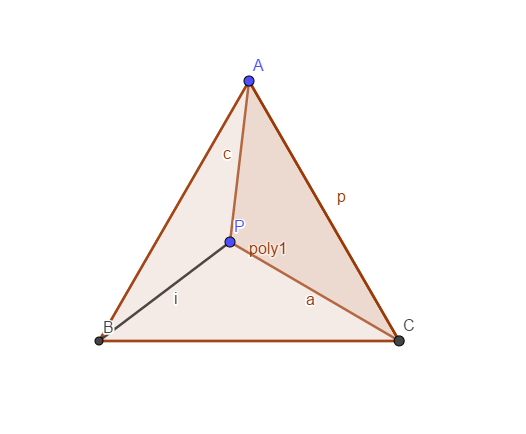
\includegraphics[scale=0.6]{Before1.jpg}
\end{figure}\\
如图所示,点P是等边三角形ABC内部一点,且
$\angle APC=117^\circ,\angle BPC=130^\circ$
,求以AP,BP,CP为边的三角形的三内角的度数。
\\\\\\
这道题目我们先分析,常规办法都不怎么好用,推平行
恐怕也不行,那么就要用到我们所说的旋转法。\\
我们将$\triangle ACP$绕顺时针旋转60度,使得AC'
与AB重合,然后连接PP',如图所示\\
\begin{figure}[ht]
    \centering
    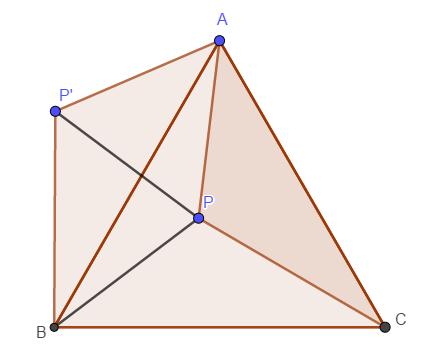
\includegraphics[scale=0.5]{After1.jpg}
\end{figure}\\
然后由于是旋转,故AP'=AP,已经有两条边相
等了,我们只要再证明除PP'=AP就能够知道
$\triangle BPP'$就是我要的三角形了。\\
为了求得PP'=AP,我要做的是求证三角形
APP'是等边三角形。由于旋转了$60^\circ$,故PAP'=
$60^\circ$,又AP'=AP从而易得$\triangle APP'$
是等边三角形,故PP'=AP',故$\triangle CPP'$就是
AP,BP,CP所组成的三角形。\\
接着就很简单了
$$\angle BPP'=\angle APB-\angle APP'=\angle APB-60^\circ=57^\circ$$
$$\angle APC=180^\circ -\angle APB-\angle BPC=108^\circ$$
$$\angle PP'B=\angle AP'B-\angle AP'P=\angle APC-60^\circ=48^\circ$$
$$\angle PBP'=180^\circ-\angle BPP'-\angle PP'B=75^\circ$$
从这个例子我们可以看到,对于存在等腰三角形,等边
三角形时,旋转使重合非常有用,对于部分习题,旋转
法可以将其变得非常易于思考。旋转这种变换,是在圆
之后的,对于部分题目旋转好用是因为圆心(旋转点)
到圆上一点处处相等,旋转后线段,角度等都不会改变,
故这是初中阶段与轴对称变换相同重要的变换。善于
用变换解题,是非常重要的。
\end{document}